\documentclass{article}
\usepackage{alltt,xcolor}
\usepackage{amsmath}
\usepackage{graphicx}

\title{Assignment 6}
\author{Nikhil Vemula, Atharva Pore, Shreeja Deshpande, Ami Sharma}

\begin{document}
  \maketitle
  \section*{Question 3}
  \begin{center}
    \begin{tabular}{c|c|c}
    size $n$ of relation {\tt S} & avg execution time to \textcolor{red}{scan} {\tt S} (in ms) &avg execution time to \textcolor{red}{sort} {\tt S} (in ms) \\ \hline
    $10^1$ &  0.021 & 0.029 \\
    $10^2$ & 0.024 &  0.056 \\
    $10^3$ & 0.166 & 0.418 \\
    $10^4$ & 1.622 & 4.491 \\
    $10^5$ & 16.460 & 55.905 \\
    $10^6$ & 147.296 & 571.115 \\
    $10^7$ & 1453.341 & 6769.971 \\
    $10^8$ & 14228.536 & 44661.351 \\
    \end{tabular}
    \end{center}
  \subsection*{Question 3a}
    \begin{enumerate}
      \item As expected the execution times are increasing with the number of records that need to sorted
      \item We observed quiksort and external merge algorithms are used while using explain analyze
      \item If the columns can be loaded into the main memory then postgres is applying quicksort the sort the values or else external sorting is being applied.
    \end{enumerate}
  \subsection*{Question 3b}
  \begin{enumerate}
    \item The time complexity of external sorting is $2 * n * log_B(n)$. These numbers follow this time complexity as the number of records increases the change in the time complexity is not so significant.
    \item We also observed that increasing the buffer memory has no significant effect on the timings after certain size.
  \end{enumerate}
  \subsubsection*{64 kB}
  \begin{verbatim}
    size of relation S | avg execution time to scan S | avg execution time to sort S 
    --------------------+------------------------------+------------------------------
                     10 |                        0.011 |                        0.017
                    100 |                        0.024 |                        0.052
                   1000 |                        0.169 |                        2.408
                  10000 |                        1.872 |                        6.989
                 100000 |                       14.371 |                       65.995
                1000000 |                      139.603 |                      915.788
               10000000 |                     1455.784 |                    10255.120
              100000000 |                    14460.073 |                   138792.104
    (8 rows)
  \end{verbatim}
  \subsubsection*{4 MB}
  \begin{verbatim}
    size of relation S | avg execution time to scan S | avg execution time to sort S 
    --------------------+------------------------------+------------------------------
                     10 |                        0.010 |                        0.016
                    100 |                        0.023 |                        0.049
                   1000 |                        0.167 |                        0.418
                  10000 |                        1.620 |                        4.403
                 100000 |                       14.064 |                       50.646
                1000000 |                      142.235 |                      564.225
               10000000 |                     1452.670 |                     6729.739
              100000000 |                    17899.258 |                   100483.906
    (8 rows)
  \end{verbatim}
  \subsubsection*{32 MB}
  \begin{verbatim}
    size of relation S | avg execution time to scan S | avg execution time to sort S 
    --------------------+------------------------------+------------------------------
                     10 |                        0.016 |                        0.019
                    100 |                        0.024 |                        0.051
                   1000 |                        0.178 |                        0.456
                  10000 |                        1.559 |                        4.234
                 100000 |                       14.388 |                       45.427
                1000000 |                      143.978 |                      611.464
               10000000 |                     1452.079 |                     6247.639
              100000000 |                    14355.261 |                    73248.857
    (8 rows)
  \end{verbatim}
  \subsubsection*{256 MB}
  \begin{verbatim}
    size of relation S | avg execution time to scan S | avg execution time to sort S 
    --------------------+------------------------------+------------------------------
                     10 |                        0.012 |                        0.021
                    100 |                        0.025 |                        0.053
                   1000 |                        0.169 |                        0.445
                  10000 |                        1.601 |                        4.811
                 100000 |                       14.403 |                       45.133
                1000000 |                      142.452 |                      545.493
               10000000 |                     1453.586 |                     6516.514
              100000000 |                    14318.139 |                    68162.534
    (8 rows)
    
  \end{verbatim}

  \subsection*{Question 3b}
  \begin{enumerate}
    \item Creating an index on the column has reduced the timings nearly by 80\%
    \item The time for creating the index with the number of records.
  \end{enumerate}
  \begin{verbatim}
    VACUUM
  size S  | create time for index (in ms) | time for range query (in ms) 
----------+-------------------------------+------------------------------
       10 |                         0.228 |                        0.022
      100 |                         0.372 |                        0.040
     1000 |                         2.373 |                        0.229
    10000 |                        21.508 |                        1.944
   100000 |                       288.745 |                       21.028
  1000000 |                      4411.057 |                      218.698
 10000000 |                     58181.511 |                     2380.300
(7 rows)
  \end{verbatim}
  \section*{Question 4}
  \subsection*{Question 4a}
  \begin{verbatim}
    VACUUM
 size of relation S | avg execution time to scan S | avg execution time to de-duplicate S 
--------------------+------------------------------+--------------------------------------
                 10 |                        0.009 |                                0.042
                100 |                        0.021 |                                0.065
               1000 |                        0.181 |                                0.438
              10000 |                        1.632 |                                4.557
             100000 |                       14.944 |                               49.861
            1000000 |                      148.068 |                              712.393
           10000000 |                     1511.463 |                             7415.293
          100000000 |                    18350.569 |                           110487.169
(8 rows)
  \end{verbatim}
  \subsection*{Question 4b}
  \begin{verbatim}
    VACUUM
 size of relation S | avg execution time to scan S | avg execution time to de-duplicate S 
--------------------+------------------------------+--------------------------------------
                 10 |                        0.010 |                                0.030
                100 |                        0.024 |                                0.062
               1000 |                        0.185 |                                0.509
              10000 |                        1.625 |                                4.397
             100000 |                       16.357 |                               81.022
            1000000 |                      172.676 |                              806.280
           10000000 |                     1490.950 |                             7195.494
          100000000 |                    16231.462 |                            97928.250
(8 rows)
  \end{verbatim}
  \subsection*{Question 4c}
  \begin{enumerate}
    \item Both the query plans are removing the duplicates as expected.
    \item The query plans for both distinct and group by look similar with similar execution times.
  \end{enumerate}
  {\scriptsize
  \begin{verbatim}
Distinct
                                              QUERY PLAN                                               
-------------------------------------------------------------------------------------------------------
 HashAggregate  (cost=41.88..43.88 rows=200 width=4) (actual time=0.038..0.046 rows=58 loops=1)
   Group Key: x
   Batches: 1  Memory Usage: 40kB
   ->  Seq Scan on s  (cost=0.00..35.50 rows=2550 width=4) (actual time=0.007..0.015 rows=100 loops=1)
 Planning Time: 0.170 ms
 Execution Time: 0.067 ms
(6 rows)

Group by
                                              QUERY PLAN                                               
-------------------------------------------------------------------------------------------------------
 HashAggregate  (cost=41.88..43.88 rows=200 width=4) (actual time=0.033..0.041 rows=58 loops=1)
   Group Key: x
   Batches: 1  Memory Usage: 40kB
   ->  Seq Scan on s  (cost=0.00..35.50 rows=2550 width=4) (actual time=0.005..0.013 rows=100 loops=1)
 Planning Time: 0.016 ms
 Execution Time: 0.054 ms
(6 rows)
  \end{verbatim}
  }

  \section*{Question 7}
  \subsection*{Question 7a}
  If the height of the tree is {\tt h} then we need to traverse atleast for {\tt h } nodes. 
  Hence the minimum time to determine if key {\tt k} is in btree is given by $ h * block\_access\_time$
  \newline
  \newline
  \begin{center}
  $n \leq \dfrac{blockSize - blockAddress}{blockAddress + key} \leq \dfrac{8192 - 10}{10 + 8} \leq 454.5$
  \end{center}
  Hence the order of the tree $ n = 454$ 
  \newline
  \begin{center}
    $N = \dfrac{numberOfRecords}{n} = \dfrac{10^{10}}{454} = 22026431$
  \end{center}
  The number of lead nodes, $N = 22026431$
  \newline
  \begin{center}
    \begin{math}
      h = \lceil log_n(N) \rceil = \lceil log_{454}(22026431) \rceil = 3
    \end{math}
  \end{center}
  The minimum access time to check key {\tt k} in btree is $3 * 10ms = \textbf{30 ms}$

  \subsection*{Question 7b}

  We get maximum time when the height of the tree is maxium. This happens when each node is half occupied i.e $n / 2 = 454 / 2 = 227$.
  So the number of lead nodes will be $ N = 10^{10} / 227 * 2 = 44052863 / 2 = 22026431$
  \newline
  Hence the height of the tree would be $\lceil log_{227}(22026431) \rceil = 4$
  \newline
  \begin{itemize}
  \item 1 i/0 to get the root of the btree
  \item So we need to traverse in the worst case 4 times to insert the record.
  \item 1 i/o operation to insert the record into the index
  \item 1 i/o operation to insert the actual record
  \end{itemize}

  Hence the maximum time taken is $ 7 * 10 = \textbf{70 ms}$

  \subsection*{Question 7c}
  \begin{itemize}
    \item The number of nodes in the first two levels are $ n + 1 = 454 + 1 = 455$. Hence we need atleast $455 * 8192 = 3727360 $ which is nearly {\textbf{4mb}}.
    \item Similary if we need to hold 3 levels then $ 1 + 454 + 454^2 = 206571$ And this needs nearly $\textbf{1.7 GB}$ of the main memory
    \item When we store these levels in the main memory the time to access a key in the btree will be reduced as the number of I/O's will be reduced.
  \end{itemize}
  
  \section*{Question 8}
  \subsection*{Question 8a}
  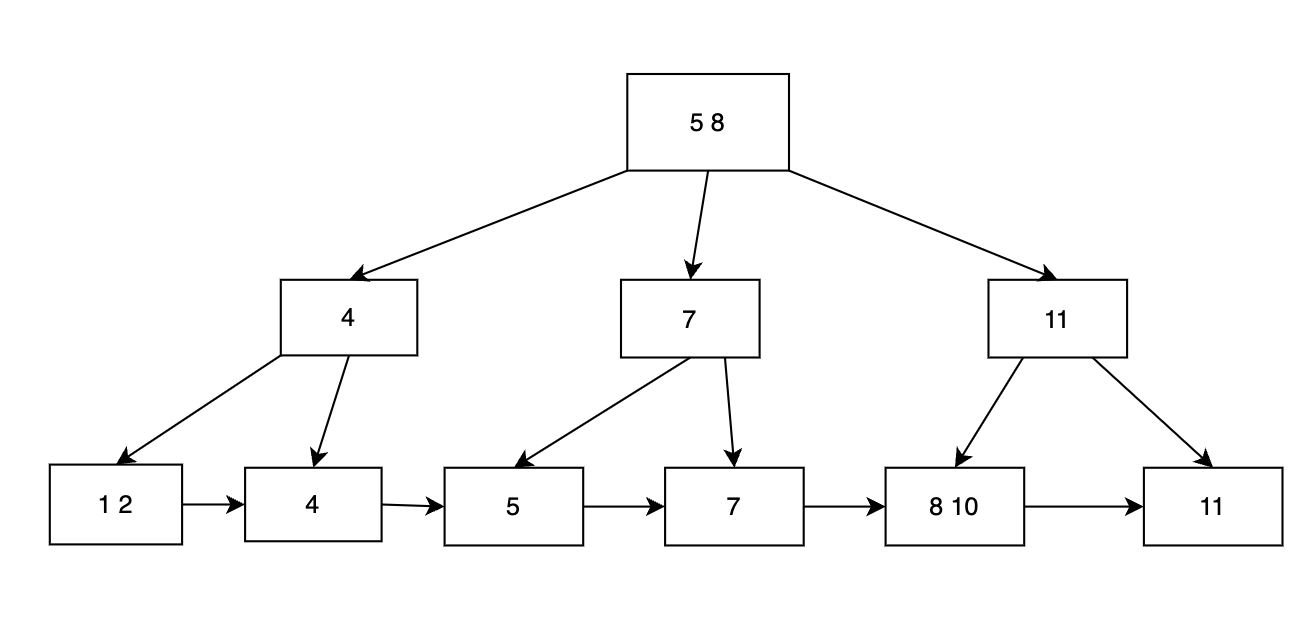
\includegraphics[scale=0.5]{insert}
  \subsection*{Question 8b}
  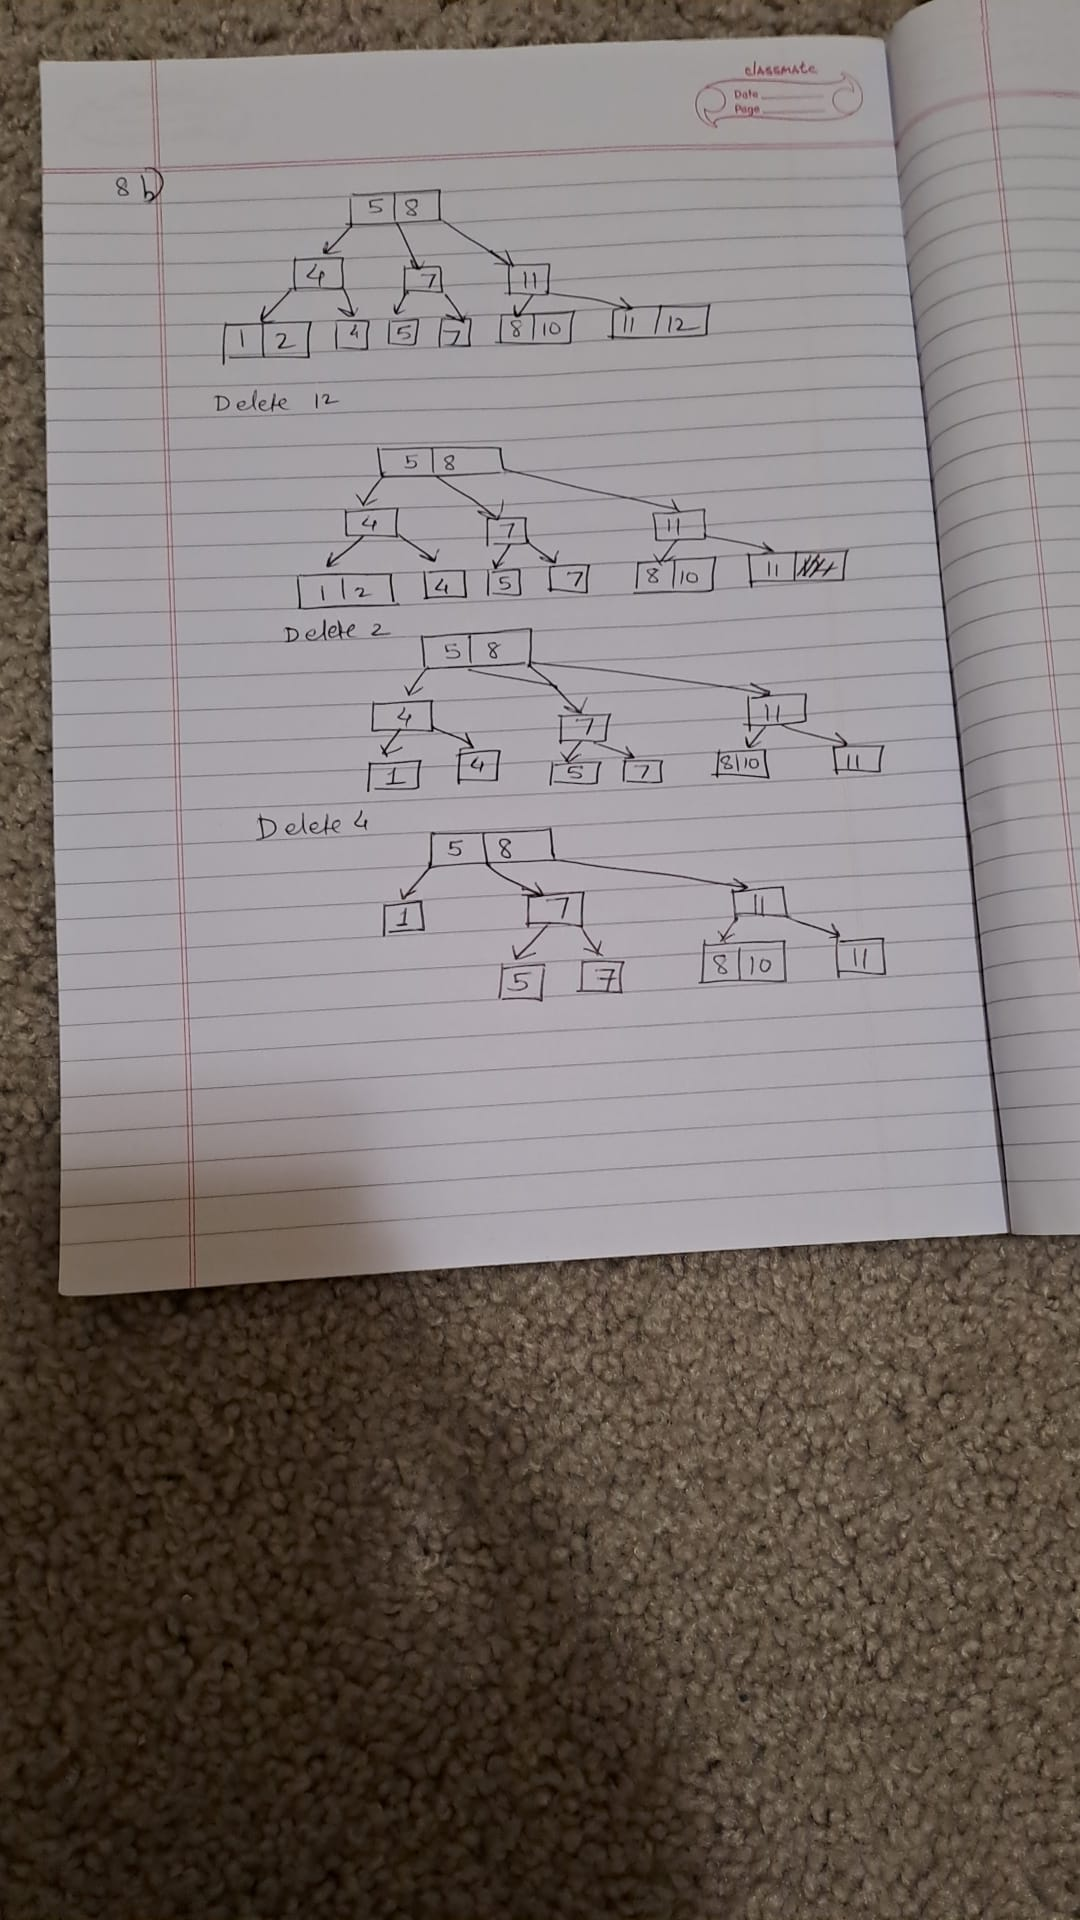
\includegraphics[scale=0.2]{8b.jpeg}
  \subsection*{Question 8c}
  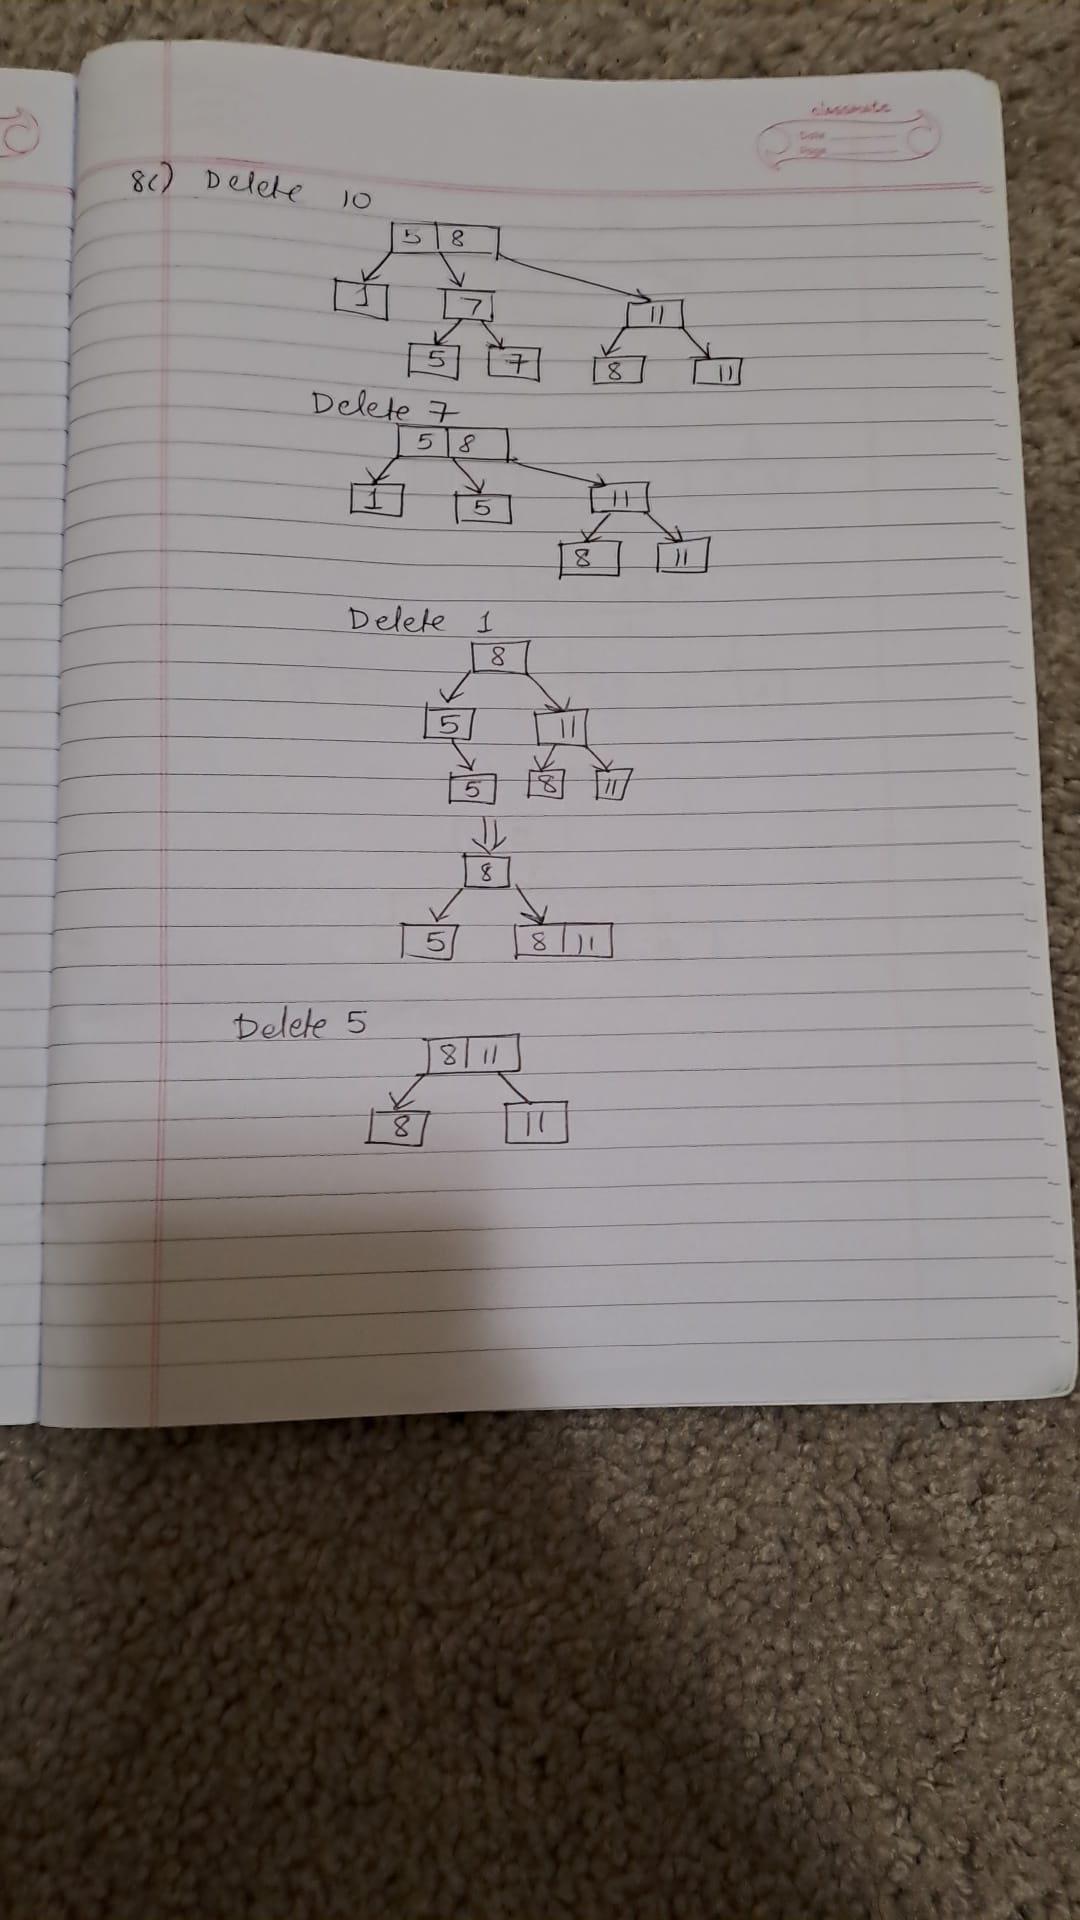
\includegraphics[scale=0.2]{8c.jpeg}
  \section*{Question 9}
  \includegraphics[scale=0.1]{9}
  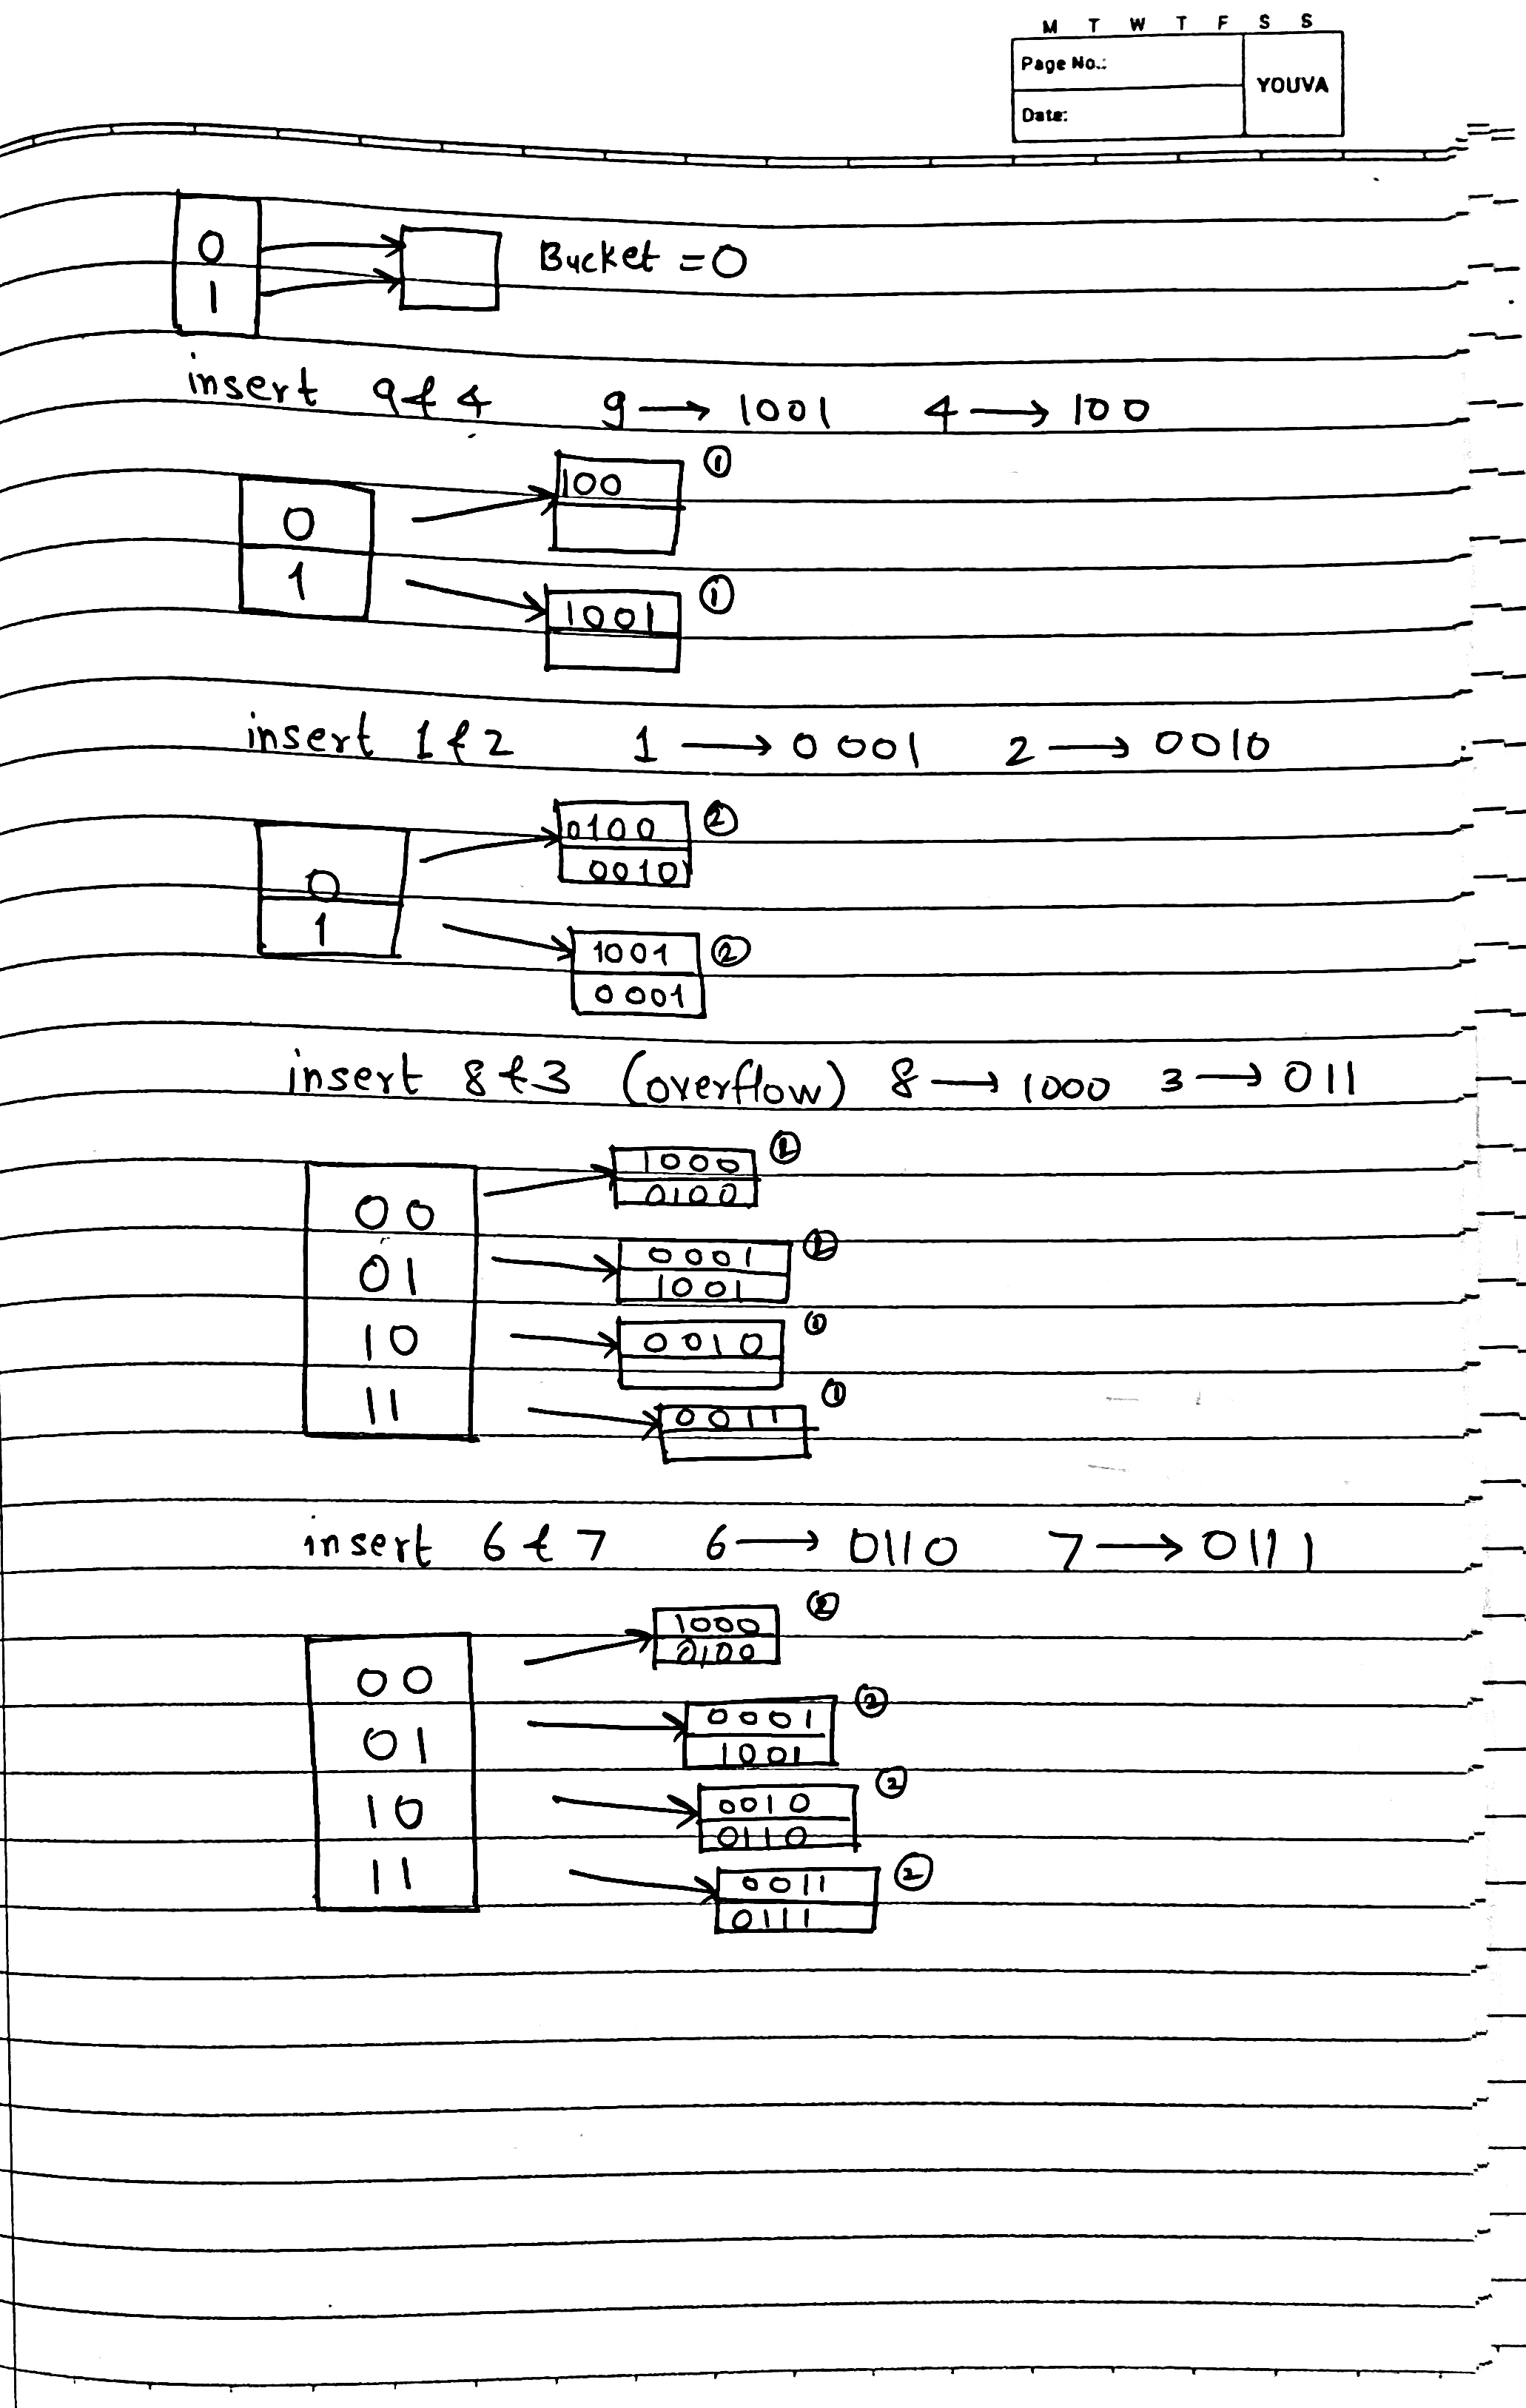
\includegraphics[scale=0.1]{hashing}
  
  
  

  \section*{Question 10}
    \subsection*{Observations}
    \begin{enumerate}
      \item With no index postgres is performing sequential scan using multiple workers to filter
      \item Creating an index on {\tt skill} column reduced the execution time by almost 50\%
      \item Didn't find any major difference in execution times between btree index and hash index. 
      \item But hash index took longer time to create on on column with more number of records
    \end{enumerate}
    \begin{center}
    {\normalsize
      \begin{tabular}{c|c|c}
      size $n$ of relation {\tt PersonSkill} & No index & With index \\ \hline
      $10^4$ & 1.007 & 0.574 \\
      $10^5$ & 9.066 & 5.825 \\
      $10^6$ & 92.875 & 45.834 \\
      $10^7$ & 973.207& 639.765\\
      \end{tabular}
    }
    \end{center}

  
    \subsection*{Query plans}
    \subsubsection*{\emph{For $10^4$ records}}
    \underline{No Index Query Plan}
    \begin{center}
      {\tiny
      \begin{alltt}
      \textcolor{blue}{
        QUERY PLAN                                                  
        -------------------------------------------------------------------------------------------------------------
         Seq Scan on personskill  (cost=0.00..163.69 rows=1802 width=4) (actual time=0.012..1.045 rows=1802 loops=1)
           Filter: (skill = 'AI'::text)
           Rows Removed by Filter: 7293
         Planning Time: 0.109 ms
         Execution Time: 1.191 ms
        (5 rows)
       }
      \end{alltt}
      }
      \end{center}
    \underline{Btree Index Query Plan}
    \begin{center}
      {\tiny
      \begin{alltt}
      \textcolor{blue}{
        QUERY PLAN                                                              
        ----------------------------------------------------------------------------
         Bitmap Heap Scan on personskill  (cost=22.25..94.78 rows=1802 width=4)  (actual time=0.067..0.465 rows=1802 loops=1)
           Recheck Cond: (skill = 'AI'::text)
           Heap Blocks: exact=50
           ->  Bitmap Index Scan on personskill_skill_idx  (cost=0.00..21.80 rows=1802 width=0) (actual time=0.054..0.054 rows=1802 loops=1)
                 Index Cond: (skill = 'AI'::text)
         Planning Time: 0.053 ms
         Execution Time: 0.620 ms
        (7 rows)
       }
      \end{alltt}
      }
      \end{center}
    \subsubsection*{\emph{For $10^5$ records}}
    \underline{No Index Query Plan}
    \begin{center}
      {\tiny
      \begin{alltt}
      \textcolor{blue}{
        QUERY PLAN                                                   
        ----------------------------------------------------------------------------------------------------------------
         Seq Scan on personskill  (cost=0.00..1621.14 rows=18123 width=4) (actual time=0.007..8.684 rows=18172 loops=1)
           Filter: (skill = 'AI'::text)
           Rows Removed by Filter: 72399
         Planning Time: 0.061 ms
         Execution Time: 9.847 ms
        (5 rows)
       }
      \end{alltt}
      }
      \end{center}
    \underline{Btree Index Query Plan}
    \begin{center}
      {\tiny
      \begin{alltt}
      \textcolor{blue}{
        QUERY PLAN                                                          
        ------------------------------------------------------------------------------------------------------------------------------
         Bitmap Heap Scan on personskill  (cost=208.75..924.28 rows=18123 width=4) (actual time=0.611..4.082 rows=18172 loops=1)
           Recheck Cond: (skill = 'AI'::text)
           Heap Blocks: exact=489
           ->  Bitmap Index Scan on skill_index  (cost=0.00..204.21 rows=18123 width=0) (actual time=0.546..0.546 rows=18172 loops=1)
                 Index Cond: (skill = 'AI'::text)
         Planning Time: 0.231 ms
         Execution Time: 5.322 ms
        (7 rows)
       }
      \end{alltt}
      }
      \end{center}
    \subsubsection*{\emph{For $10^6$ records}}
    \underline{No index Query Plan}
    \begin{center}
      {\tiny
      \begin{alltt}
      \textcolor{blue}{
        QUERY PLAN                                                     
        --------------------------------------------------------------------------------------------------------------------
         Seq Scan on personskill  (cost=0.00..16227.24 rows=183887 width=4) (actual time=0.025..81.109 rows=181384 loops=1)
           Filter: (skill = 'AI'::text)
           Rows Removed by Filter: 725355
         Planning Time: 0.040 ms
         Execution Time: 91.967 ms
        (5 rows)
       }
      \end{alltt}
      }
    \end{center}
    \underline{Btree index Query Plan}
    \begin{center}
      {\tiny
      \begin{alltt}
      \textcolor{blue}{
        QUERY PLAN                                                            
        ---------------------------------------------------------------------------------------------------------------------------------
         Bitmap Heap Scan on personskill  (cost=2031.29..9186.98 rows=181015 width=4) (actual time=6.280..38.996 rows=181384 loops=1)
           Recheck Cond: (skill = 'AI'::text)
           Heap Blocks: exact=4893
           ->  Bitmap Index Scan on skill_index  (cost=0.00..1986.04 rows=181015 width=0) (actual time=5.554..5.555 rows=181384 loops=1)
                 Index Cond: (skill = 'AI'::text)
         Planning Time: 0.238 ms
         Execution Time: 50.507 ms
        (7 rows)
       }
      \end{alltt}
      }
    \end{center}
    \subsubsection*{\emph{For $10^7$ records}}
    \underline{No index Query Plan}
    \begin{center}
      {\tiny
      \begin{alltt}
      \textcolor{blue}{
        queryplan                                                        
        ------------------------------------------------------------------------------------------------------------------------
         Seq Scan on personskill  (cost=0.00..162223.31 rows=1834672 width=4) (actual time=0.019..795.445 rows=1811314 loops=1)
           Filter: (skill = 'AI'::text)
           Rows Removed by Filter: 7253413
         Planning Time: 0.113 ms
         Execution Time: 895.138 ms
        (5 rows)
       }
      \end{alltt}
      }
    \end{center}
    \underline{Btree index Query Plan}
    \begin{center}
      {\tiny
      \begin{alltt}
      \textcolor{blue}{
        queryplan                                                               
        --------------------------------------------------------------------------------------------------------------------------------------
         Bitmap Heap Scan on personskill  (cost=20527.37..92377.13 rows=1834701 width=4) (actual time=77.331..499.683 rows=1811314 loops=1)
           Recheck Cond: (skill = 'AI'::text)
           Heap Blocks: exact=48916
           ->  Bitmap Index Scan on skill_index  (cost=0.00..20068.69 rows=1834701 width=0) (actual time=68.578..68.578 rows=1811314 loops=1)
                 Index Cond: (skill = 'AI'::text)
         Planning Time: 0.286 ms
         Execution Time: 603.233 ms
        (7 rows)
       }
      \end{alltt}
      }
    \end{center}

    \section*{Question 11}
    \subsection*{Observations}
    \begin{enumerate}
      \item As expected adding an btree index helped for range queries. But!
      \item If the stats for a given range are high then postgres is performing a sequential scan though index is available.
      \item For smaller range, the execution time is nearly constant even when the number of records increased
      \item Interestingly larger range performs slightly better than medium range as it covers the whole table?
    \end{enumerate}
    \subsubsection*{Small Range}
    \begin{center}
      {\normalsize
        \begin{tabular}{c|c|c}
        size $n$ of relation {\tt worksFor} & No index & With index \\ \hline
        $10^4$ & 0.961 & 0.020 \\
        $10^5$ & 8.45 & 0.021 \\
        $10^6$ & 37.561 & 0.022 \\
        $10^7$ & 279.965 & 0.021\\
        \end{tabular}
      }
      \end{center}

      \subsubsection*{Medium Range}
      \begin{center}
        {\normalsize
          \begin{tabular}{c|c|c}
          size $n$ of relation {\tt worksFor} & No index & With index \\ \hline
          $10^4$ & 1.726 & 1.552\\
          $10^5$ & 24.065 & 23.626\\
          $10^6$ & 216.149 &  203.814\\
          $10^7$ & 1970.034 & 1953.22\\
          \end{tabular}
        }
        \end{center}
    
        \subsubsection*{Large Range}
    \begin{center}
      {\normalsize
        \begin{tabular}{c|c|c}
        size $n$ of relation {\tt worksFor} & No index & With index \\ \hline
        $10^4$ & 2.565 & 2.409\\
        $10^5$ & 20.516 & 21.637\\
        $10^6$ & 196.60 &  205.833\\
        $10^7$ & 1807.410 & 1783.657\\
        \end{tabular}
      }
      \end{center}

    \subsection*{Query Plans}
    \subsubsection*{Small Range}
    \subsubsection*{\emph{For $10^4$ records}}
    \underline{No Index Query Plan}
    \begin{center}
      {\tiny
      \begin{alltt}
      \textcolor{blue}{
        QUERY PLAN                                             
        ----------------------------------------------------------------------------------------------------
         Seq Scan on worksfor  (cost=0.00..205.00 rows=1 width=4) (actual time=0.009..0.964 rows=1 loops=1)
           Filter: ((10000 <= salary) AND (salary <= 10000))
           Rows Removed by Filter: 9999
         Planning Time: 0.148 ms
         Execution Time: 0.976 ms
        (5 rows)
       }
      \end{alltt}
      }
    \end{center}
    \underline{With Index Query Plan}
    \begin{center}
      {\tiny
      \begin{alltt}
      \textcolor{blue}{
        QUERY PLAN                                                          
        ------------------------------------------------------------------------------------------------------------------------------
         Index Scan using worksfor_salary_idx on worksfor  (cost=0.29..8.32 rows=2 width=4) (actual time=0.007..0.008 rows=1 loops=1)
           Index Cond: ((salary >= 10000) AND (salary <= 10000))
         Planning Time: 0.128 ms
         Execution Time: 0.019 ms
        (4 rows)
       }
      \end{alltt}
      }
    \end{center}
    \subsubsection*{\emph{For $10^5$ records}}
    \underline{No Index Query Plan}
    \begin{center}
      {\tiny
      \begin{alltt}
      \textcolor{blue}{
        QUERY PLAN                                              
        -----------------------------------------------------------------------------------------------------
         Seq Scan on worksfor  (cost=0.00..2041.00 rows=1 width=4) (actual time=0.008..8.500 rows=3 loops=1)
           Filter: ((10000 <= salary) AND (salary <= 10000))
           Rows Removed by Filter: 99997
         Planning Time: 0.071 ms
         Execution Time: 8.513 ms
        (5 rows)
       }
      \end{alltt}
      }
    \end{center}
    \underline{With Index Query Plan}
    \begin{center}
      {\tiny
      \begin{alltt}
      \textcolor{blue}{
        QUERY PLAN                                                          
        ------------------------------------------------------------------------------------------------------------------------------
         Index Scan using worksfor_salary_idx on worksfor  (cost=0.29..8.33 rows=2 width=4) (actual time=0.007..0.008 rows=3 loops=1)
           Index Cond: ((salary >= 10000) AND (salary <= 10000))
         Planning Time: 0.453 ms
         Execution Time: 0.021 ms
        (4 rows)
       }
      \end{alltt}
      }
    \end{center}
    \subsubsection*{\emph{For $10^6$ records}}
    \underline{No Index Query Plan}
    \begin{center}
      {\tiny
      \begin{alltt}
      \textcolor{blue}{
        QUERY PLAN                                                       
        -----------------------------------------------------------------------------------------------------------------------
         Gather  (cost=1000.00..13620.10 rows=1 width=8) (actual time=0.135..37.094 rows=4 loops=1)
           Workers Planned: 2
           Workers Launched: 2
           ->  Parallel Seq Scan on worksfor  (cost=0.00..12620.00 rows=1 width=8) (actual time=19.437..31.110 rows=1 loops=3)
                 Filter: ((100 <= salary) AND (salary <= 100))
                 Rows Removed by Filter: 333332
         Planning Time: 0.075 ms
         Execution Time: 37.107 ms
        (8 rows)
       }
      \end{alltt}
      }
    \end{center}
    \underline{With Index Query Plan}
    \begin{center}
      {\tiny
      \begin{alltt}
      \textcolor{blue}{
        QUERY PLAN                                                          
        ------------------------------------------------------------------------------------------------------------------------------
         Index Scan using worksfor_salary_idx on worksfor  (cost=0.42..8.46 rows=2 width=8) (actual time=0.014..0.016 rows=4 loops=1)
           Index Cond: ((salary >= 100) AND (salary <= 100))
         Planning Time: 0.291 ms
         Execution Time: 0.027 ms
        (4 rows)
       }
      \end{alltt}
      }
    \end{center}

    \subsubsection*{\emph{For $10^7$ records}}
    \underline{No Index Query Plan}
    \begin{center}
      {\tiny
      \begin{alltt}
      \textcolor{blue}{
        QUERY PLAN                                                        
        --------------------------------------------------------------------------------------------------------------------------
         Gather  (cost=1000.00..127195.82 rows=1 width=8) (actual time=0.173..282.248 rows=1 loops=1)
           Workers Planned: 2
           Workers Launched: 2
           ->  Parallel Seq Scan on worksfor  (cost=0.00..126195.72 rows=1 width=8) (actual time=182.311..275.322 rows=0 loops=3)
                 Filter: ((100 <= salary) AND (salary <= 100))
                 Rows Removed by Filter: 3333333
         Planning Time: 0.130 ms
         Execution Time: 282.266 ms
        (8 rows)
       }
      \end{alltt}
      }
    \end{center}
    \underline{With Index Query Plan}
    \begin{center}
      {\tiny
      \begin{alltt}
      \textcolor{blue}{
        QUERY PLAN                                                          
        ------------------------------------------------------------------------------------------------------------------------------
         Index Scan using worksfor_salary_idx on worksfor  (cost=0.43..8.50 rows=3 width=8) (actual time=0.014..0.015 rows=1 loops=1)
           Index Cond: ((salary >= 100) AND (salary <= 100))
         Planning Time: 0.501 ms
         Execution Time: 0.027 ms
        (4 rows)
       }
      \end{alltt}
      }
    \end{center}

    \subsubsection*{Medium Range}
    \subsubsection*{\emph{For $10^4$ records}}
    \underline{No Index Query Plan}
    \begin{center}
      {\tiny
      \begin{alltt}
      \textcolor{blue}{
        QUERY PLAN                                                
        ----------------------------------------------------------------------------------------------------------
         Seq Scan on worksfor  (cost=0.00..205.00 rows=4961 width=4) (actual time=0.014..1.688 rows=4955 loops=1)
           Filter: ((10000 <= salary) AND (salary <= 50186992))
           Rows Removed by Filter: 5045
         Planning Time: 0.073 ms
         Execution Time: 2.182 ms
        (5 rows)
       }
      \end{alltt}
      }
    \end{center}
    \underline{With Index Query Plan}
    \begin{center}
      {\tiny
      \begin{alltt}
      \textcolor{blue}{
        QUERY PLAN                                                              
        --------------------------------------------------------------------------------------------------------------------------------------
         Index Scan using worksfor_salary_idx on worksfor  (cost=0.29..186.53 rows=4962 width=4) (actual time=0.018..1.170 rows=4955 loops=1)
           Index Cond: ((salary >= 10000) AND (salary <= 50186992))
         Planning Time: 0.090 ms
         Execution Time: 1.531 ms
        (4 rows)
       }
      \end{alltt}
      }
    \end{center}
    \subsubsection*{\emph{For $10^5$ records}}
    \underline{No Index Query Plan}
    \begin{center}
      {\tiny
      \begin{alltt}
      \textcolor{blue}{
        QUERY PLAN                                                  
        --------------------------------------------------------------------------------------------------------------
         Seq Scan on worksfor  (cost=0.00..2291.00 rows=33330 width=4) (actual time=0.008..19.839 rows=50095 loops=1)
           Filter: ((10000 <= salary) AND ((salary)::numeric <= 499212216.5))
           Rows Removed by Filter: 49905
         Planning Time: 0.038 ms
         Execution Time: 23.056 ms
        (5 rows)
       }
      \end{alltt}
      }
    \end{center}
    \underline{With Index Query Plan}
    \begin{center}
      {\tiny
      \begin{alltt}
      \textcolor{blue}{
        QUERY PLAN                                                  
        --------------------------------------------------------------------------------------------------------------
         Seq Scan on worksfor  (cost=0.00..2291.00 rows=33333 width=4) (actual time=0.010..20.457 rows=50095 loops=1)
           Filter: ((10000 <= salary) AND ((salary)::numeric <= 499212216.5))
           Rows Removed by Filter: 49905
         Planning Time: 0.083 ms
         Execution Time: 23.758 ms
        (5 rows)
       }
      \end{alltt}
      }
    \end{center}
    \subsubsection*{\emph{For $10^6$ records}}
    \underline{No Index Query Plan}
    \begin{center}
      {\tiny
      \begin{alltt}
      \textcolor{blue}{
        QUERY PLAN                                                    
        ------------------------------------------------------------------------------------------------------------------
         Seq Scan on worksfor  (cost=0.00..23870.00 rows=333300 width=8) (actual time=0.010..179.810 rows=500077 loops=1)
           Filter: ((100 <= salary) AND ((salary)::numeric <= 49956718.44850))
           Rows Removed by Filter: 499923
         Planning Time: 0.048 ms
         Execution Time: 209.021 ms
        (5 rows)
       }
      \end{alltt}
      }
    \end{center}
    \underline{With Index Query Plan}
    \begin{center}
      {\tiny
      \begin{alltt}
      \textcolor{blue}{
        QUERY PLAN                                                    
        ------------------------------------------------------------------------------------------------------------------
         Seq Scan on worksfor  (cost=0.00..23870.00 rows=333333 width=8) (actual time=0.013..211.058 rows=500077 loops=1)
           Filter: ((100 <= salary) AND ((salary)::numeric <= 49956718.44850))
           Rows Removed by Filter: 499923
         Planning Time: 0.116 ms
         Execution Time: 240.352 ms
        (5 rows)
       }
      \end{alltt}
      }
    \end{center}

    \subsubsection*{\emph{For $10^7$ records}}
    \underline{No Index Query Plan}
    \begin{center}
      {\tiny
      \begin{alltt}
      \textcolor{blue}{
        QUERY PLAN                                                      
        ----------------------------------------------------------------------------------------------------------------------
         Seq Scan on worksfor  (cost=0.00..238697.01 rows=3333038 width=8) (actual time=0.129..1717.734 rows=5000037 loops=1)
           Filter: ((100 <= salary) AND ((salary)::numeric <= 500082613.5282))
           Rows Removed by Filter: 4999963
         Planning Time: 0.072 ms
         Execution Time: 1985.666 ms
        (5 rows)
       }
      \end{alltt}
      }
    \end{center}
    \underline{With Index Query Plan}
    \begin{center}
      {\tiny
      \begin{alltt}
      \textcolor{blue}{
        QUERY PLAN                                                      
        ----------------------------------------------------------------------------------------------------------------------
         Seq Scan on worksfor  (cost=0.00..238695.00 rows=3333333 width=8) (actual time=0.010..1737.548 rows=5000037 loops=1)
           Filter: ((100 <= salary) AND ((salary)::numeric <= 500082613.5282))
           Rows Removed by Filter: 4999963
         Planning Time: 0.081 ms
         Execution Time: 2017.289 ms
        (5 rows)
       }
      \end{alltt}
      }
    \end{center}


    \subsubsection*{Large Range}
    \subsubsection*{\emph{For $10^4$ records}}
    \underline{No Index Query Plan}
    \begin{center}
      {\tiny
      \begin{alltt}
      \textcolor{blue}{
        QUERY PLAN                                                 
        -----------------------------------------------------------------------------------------------------------
         Seq Scan on worksfor  (cost=0.00..205.00 rows=9998 width=4) (actual time=0.010..1.891 rows=10000 loops=1)
           Filter: ((10000 <= salary) AND (salary <= 99980000))
         Planning Time: 0.052 ms
         Execution Time: 2.656 ms
        (4 rows)
       }
      \end{alltt}
      }
    \end{center}
    \underline{With Index Query Plan}
    \begin{center}
      {\tiny
      \begin{alltt}
      \textcolor{blue}{
        QUERY PLAN                                                 
        ------------------------------------------------------------------------------------------------------------
         Seq Scan on worksfor  (cost=0.00..205.00 rows=10000 width=4) (actual time=0.013..1.734 rows=10000 loops=1)
           Filter: ((10000 <= salary) AND (salary <= 99980000))
         Planning Time: 0.211 ms
         Execution Time: 2.500 ms
        (4 rows)
       }
      \end{alltt}
      }
    \end{center}
    \subsubsection*{\emph{For $10^5$ records}}
    \underline{No Index Query Plan}
    \begin{center}
      {\tiny
      \begin{alltt}
      \textcolor{blue}{
        QUERY PLAN                                                   
        ---------------------------------------------------------------------------------------------------------------
         Seq Scan on worksfor  (cost=0.00..2041.00 rows=99980 width=4) (actual time=0.010..14.724 rows=100000 loops=1)
           Filter: ((10000 <= salary) AND (salary <= 1000000000))
         Planning Time: 0.143 ms
         Execution Time: 21.192 ms
        (4 rows)
       }
      \end{alltt}
      }
    \end{center}
    \underline{With Index Query Plan}
    \begin{center}
      {\tiny
      \begin{alltt}
      \textcolor{blue}{
        QUERY PLAN                                                   
        ----------------------------------------------------------------------------------------------------------------
         Seq Scan on worksfor  (cost=0.00..2041.00 rows=100000 width=4) (actual time=0.011..14.475 rows=100000 loops=1)
           Filter: ((10000 <= salary) AND (salary <= 1000000000))
         Planning Time: 0.227 ms
         Execution Time: 20.928 ms
        (4 rows)
       }
      \end{alltt}
      }
    \end{center}
    \subsubsection*{\emph{For $10^6$ records}}
    \underline{No Index Query Plan}
    \begin{center}
      {\tiny
      \begin{alltt}
      \textcolor{blue}{
        QUERY PLAN                                                     
        -------------------------------------------------------------------------------------------------------------------
         Seq Scan on worksfor  (cost=0.00..21370.00 rows=999800 width=8) (actual time=0.024..136.545 rows=1000000 loops=1)
           Filter: ((100 <= salary) AND (salary <= 100000000))
         Planning Time: 0.129 ms
         Execution Time: 194.728 ms
        (4 rows)
       }
      \end{alltt}
      }
    \end{center}
    \underline{With Index Query Plan}
    \begin{center}
      {\tiny
      \begin{alltt}
      \textcolor{blue}{
        QUERY PLAN                                                     
        --------------------------------------------------------------------------------------------------------------------
         Seq Scan on worksfor  (cost=0.00..21370.00 rows=1000000 width=8) (actual time=0.009..135.051 rows=1000000 loops=1)
           Filter: ((100 <= salary) AND (salary <= 100000000))
         Planning Time: 0.213 ms
         Execution Time: 192.895 ms
        (4 rows)
       }
      \end{alltt}
      }
    \end{center}
    \subsubsection*{\emph{For $10^7$ records}}
    \underline{No Index Query Plan}
    \begin{center}
      {\tiny
      \begin{alltt}
      \textcolor{blue}{
        QUERY PLAN                                                       
        -----------------------------------------------------------------------------------------------------------------------
         Seq Scan on worksfor  (cost=0.00..213696.73 rows=9998115 width=8) (actual time=0.030..1298.063 rows=10000000 loops=1)
           Filter: ((100 <= salary) AND (salary <= 1000000000))
         Planning Time: 0.064 ms
         Execution Time: 1837.039 ms
        (4 rows)
       }
      \end{alltt}
      }
    \end{center}
    \underline{With Index Query Plan}
    \begin{center}
      {\tiny
      \begin{alltt}
      \textcolor{blue}{
        QUERY PLAN                                                       
        ------------------------------------------------------------------------------------------------------------------------
         Seq Scan on worksfor  (cost=0.00..213695.00 rows=10000000 width=8) (actual time=0.010..1345.495 rows=10000000 loops=1)
           Filter: ((100 <= salary) AND (salary <= 1000000000))
         Planning Time: 0.811 ms
         Execution Time: 1898.255 ms
        (4 rows)
       }
      \end{alltt}
      }
    \end{center}

  \section*{Question 12}
  \subsection*{Observations}
  \begin{center}
    \begin{enumerate}
      \item Creating an composite index (pid, skill) helped with query very effectively
      \item Postgres is performing Index only scan as the select clause is readily available in the index itself. Hence it is blazingly fast even for large number of records
    \end{enumerate}
    {\normalsize
      \begin{tabular}{c|c|c}
      size $n$ of relation {\tt PersonSkill} & No index & With index \\ \hline
      $10^4$ & 0.776 & 0.025\\
      $10^5$ & 6.859 &  0.027\\
      $10^6$ & 31.71 &  0.028\\
      $10^7$ & 360.053 & 0.028\\
      \end{tabular}
    }
    \end{center}
  \subsection*{Query Plans}
  \subsubsection*{\emph{For $10^4$ records}}
    \underline{No Index Query Plan}
    \begin{center}
      {\tiny
      \begin{alltt}
      \textcolor{blue}{
        QUERY PLAN                                               
        --------------------------------------------------------------------------------------------------------
         Seq Scan on personskill  (cost=0.00..184.21 rows=1 width=14) (actual time=0.016..0.786 rows=1 loops=1)
           Filter: ((pid = 101) AND (skill = 'AI'::text))
           Rows Removed by Filter: 9013
         Planning Time: 0.094 ms
         Execution Time: 0.797 ms
        (5 rows)
       }
      \end{alltt}
      }
    \end{center}
    \underline{With Index Query Plan}
    \begin{center}
      {\tiny
      \begin{alltt}
      \textcolor{blue}{
        QUERY PLAN                                                                  
        ---------------------------------------------------------------------------------------------------------------------------------------------
         Index Only Scan using personskill_pid_skill_idx on personskill  (cost=0.29..4.30 rows=1 width=14) (actual time=0.046..0.047 rows=1 loops=1)
           Index Cond: ((pid = 101) AND (skill = 'AI'::text))
           Heap Fetches: 0
         Planning Time: 0.234 ms
         Execution Time: 0.058 ms
        (5 rows)
       }
      \end{alltt}
      }
    \end{center}
    \subsubsection*{\emph{For $10^5$ records}}
    \underline{No Index Query Plan}
    \begin{center}
      {\tiny
      \begin{alltt}
      \textcolor{blue}{
        QUERY PLAN                                                
        ---------------------------------------------------------------------------------------------------------
         Seq Scan on personskill  (cost=0.00..1847.31 rows=1 width=14) (actual time=0.017..7.034 rows=1 loops=1)
           Filter: ((pid = 102) AND (skill = 'AI'::text))
           Rows Removed by Filter: 90553
         Planning Time: 0.053 ms
         Execution Time: 7.047 ms
        (5 rows)
       }
      \end{alltt}
      }
    \end{center}
    \underline{With Index Query Plan}
    \begin{center}
      {\tiny
      \begin{alltt}
      \textcolor{blue}{
        QUERY PLAN                                                                  
        ---------------------------------------------------------------------------------------------------------------------------------------------
         Index Only Scan using personskill_pid_skill_idx on personskill  (cost=0.42..4.44 rows=1 width=14) (actual time=0.063..0.064 rows=1 loops=1)
           Index Cond: ((pid = 102) AND (skill = 'AI'::text))
           Heap Fetches: 0
         Planning Time: 0.335 ms
         Execution Time: 0.076 ms
        (5 rows)
       }
      \end{alltt}
      }
    \end{center}
    \subsubsection*{\emph{For $10^6$ records}}
    \underline{No Index Query Plan}
    \begin{center}
      {\tiny
      \begin{alltt}
      \textcolor{blue}{
        QUERY PLAN                                                         
        ---------------------------------------------------------------------------------------------------------------------------
         Gather  (cost=1000.00..11557.49 rows=1 width=14) (actual time=0.183..31.747 rows=1 loops=1)
           Workers Planned: 2
           Workers Launched: 2
           ->  Parallel Seq Scan on personskill  (cost=0.00..10557.39 rows=1 width=14) (actual time=15.999..25.964 rows=0 loops=3)
                 Filter: ((pid = 160) AND (skill = 'AI'::text))
                 Rows Removed by Filter: 302154
         Planning Time: 0.048 ms
         Execution Time: 31.761 ms
        (8 rows)
       }
      \end{alltt}
      }
    \end{center}
    \underline{With Index Query Plan}
    \begin{center}
      {\tiny
      \begin{alltt}
      \textcolor{blue}{
        QUERY PLAN                                                                  
        ---------------------------------------------------------------------------------------------------------------------------------------------
         Index Only Scan using personskill_pid_skill_idx on personskill  (cost=0.42..4.44 rows=1 width=14) (actual time=0.055..0.056 rows=1 loops=1)
           Index Cond: ((pid = 160) AND (skill = 'AI'::text))
           Heap Fetches: 0
         Planning Time: 0.254 ms
         Execution Time: 0.068 ms
        (5 rows)
       }
      \end{alltt}
      }
    \end{center}
    \subsubsection*{\emph{For $10^7$ records}}
    \underline{No Index Query Plan}
    \begin{center}
      {\tiny
      \begin{alltt}
      \textcolor{blue}{
        QUERY PLAN                                                          
        ------------------------------------------------------------------------------------------------------------------------------
         Gather  (cost=1000.00..106540.20 rows=1 width=14) (actual time=0.708..366.035 rows=1 loops=1)
           Workers Planned: 2
           Workers Launched: 2
           ->  Parallel Seq Scan on personskill  (cost=0.00..105540.10 rows=1 width=14) (actual time=233.990..354.330 rows=0 loops=3)
                 Filter: ((pid = 120) AND (skill = 'AI'::text))
                 Rows Removed by Filter: 3020812
         Planning Time: 0.049 ms
         Execution Time: 366.052 ms
        (8 rows)
       }
      \end{alltt}
      }
    \end{center}
    \underline{With Index Query Plan}
    \begin{center}
      {\tiny
      \begin{alltt}
      \textcolor{blue}{
        QUERY PLAN                                                                  
        ---------------------------------------------------------------------------------------------------------------------------------------------
         Index Only Scan using personskill_pid_skill_idx on personskill  (cost=0.43..4.45 rows=1 width=14) (actual time=0.012..0.013 rows=1 loops=1)
           Index Cond: ((pid = 100) AND (skill = 'AI'::text))
           Heap Fetches: 0
         Planning Time: 0.055 ms
         Execution Time: 0.025 ms
        (5 rows)
       }
      \end{alltt}
      }
    \end{center}

    \section*{Question 13}
    \subsection*{\underline{Semi Join}}
    \subsection*{Observations}
    \begin{center}
      \begin{enumerate}
        \item Created composite index (skill, pid) on personSkill to make use of index scan only.
        \item This index is used to generate the hash for hash semi join on person table
        \item We observed no significant improvement. We only got minor improvedment due to the index only scan being used for person skill to construct the sub plan hash
        \item This is expected considering the semi join and anti semi join are implemented in linear time complexity already.
      \end{enumerate}
      \vspace*{10pt}
      {\normalsize
        \begin{tabular}{c|c|c}
        size $n$ of relation {\tt PersonSkill} & No index & With index \\ \hline
        $10^4$ & 4.021 & 3.262\\
        $10^5$ & 38.645 &  32.764\\
        $10^6$ & 523.410 &  457.729\\
        $10^7$ & 9592.538 & 8720.626 \\
        \end{tabular}
      }
      \end{center}
    \subsection*{Query Plans}
    \subsubsection*{\emph{For $10^4$ records}}
    \underline{No Index Query Plan}
    \begin{center}
      {\tiny
      \begin{alltt}
      \textcolor{blue}{
        QUERY PLAN                                                        
        -------------------------------------------------------------------------------------------------------------------------
         Hash Semi Join  (cost=185.39..399.72 rows=2896 width=8) (actual time=1.415..3.828 rows=1843 loops=1)
           Hash Cond: (person.pid = personskill.pid)
           ->  Seq Scan on person  (cost=0.00..145.00 rows=10000 width=8) (actual time=0.012..0.967 rows=10000 loops=1)
           ->  Hash  (cost=162.35..162.35 rows=1843 width=4) (actual time=1.395..1.396 rows=1843 loops=1)
                 Buckets: 2048  Batches: 1  Memory Usage: 81kB
                 ->  Seq Scan on personskill  (cost=0.00..162.35 rows=1843 width=4) (actual time=0.008..1.074 rows=1843 loops=1)
                       Filter: (skill = 'AI'::text)
                       Rows Removed by Filter: 7225
         Planning Time: 0.373 ms
         Execution Time: 3.973 ms
        (10 rows)
       }
      \end{alltt}
      }
    \end{center}
    \underline{With Index Query Plan}
    \begin{center}
      {\tiny
      \begin{alltt}
      \textcolor{blue}{
        QUERY PLAN                                                                           
        ---------------------------------------------------------------------------------------------------------------------------------------------------------------
         Hash Semi Join  (cost=87.57..301.90 rows=2896 width=8) (actual time=0.584..3.335 rows=1843 loops=1)
           Hash Cond: (person.pid = personskill.pid)
           ->  Seq Scan on person  (cost=0.00..145.00 rows=10000 width=8) (actual time=0.009..1.032 rows=10000 loops=1)
           ->  Hash  (cost=64.54..64.54 rows=1843 width=4) (actual time=0.566..0.567 rows=1843 loops=1)
                 Buckets: 2048  Batches: 1  Memory Usage: 81kB
                 ->  Index Only Scan using personskill_skill_pid_idx on personskill  (cost=0.29..64.54 rows=1843 width=4) (actual time=0.023..0.303 rows=1843 loops=1)
                       Index Cond: (skill = 'AI'::text)
                       Heap Fetches: 0
         Planning Time: 0.341 ms
         Execution Time: 3.548 ms
        (10 rows)
       }
      \end{alltt}
      }
    \end{center}
    \subsubsection*{\emph{For $10^5$ records}}
    \underline{No Index Query Plan}
    \begin{center}
      {\tiny
      \begin{alltt}
      \textcolor{blue}{
        QUERY PLAN                                                         
        ----------------------------------------------------------------------------------------------------------------------------
         Hash Semi Join  (cost=1849.03..3953.87 rows=32270 width=8) (actual time=12.274..37.028 rows=18119 loops=1)
           Hash Cond: (person.pid = personskill.pid)
           ->  Seq Scan on person  (cost=0.00..1443.00 rows=100000 width=8) (actual time=0.009..8.995 rows=100000 loops=1)
           ->  Hash  (cost=1623.28..1623.28 rows=18060 width=4) (actual time=12.244..12.245 rows=18119 loops=1)
                 Buckets: 32768  Batches: 1  Memory Usage: 893kB
                 ->  Seq Scan on personskill  (cost=0.00..1623.28 rows=18060 width=4) (actual time=0.018..9.072 rows=18119 loops=1)
                       Filter: (skill = 'AI'::text)
                       Rows Removed by Filter: 72543
         Planning Time: 0.306 ms
         Execution Time: 38.719 ms
        (10 rows)
       }
      \end{alltt}
      }
    \end{center}
    \underline{With Index Query Plan}
    \begin{center}
      {\tiny
      \begin{alltt}
      \textcolor{blue}{
        QUERY PLAN                                                                            
        ------------------------------------------------------------------------------------------------------------------------------------------------------------------
         Hash Semi Join  (cost=826.22..2931.06 rows=32270 width=8) (actual time=6.257..31.265 rows=18119 loops=1)
           Hash Cond: (person.pid = personskill.pid)
           ->  Seq Scan on person  (cost=0.00..1443.00 rows=100000 width=8) (actual time=0.006..8.948 rows=100000 loops=1)
           ->  Hash  (cost=600.47..600.47 rows=18060 width=4) (actual time=6.233..6.234 rows=18119 loops=1)
                 Buckets: 32768  Batches: 1  Memory Usage: 893kB
                 ->  Index Only Scan using personskill_skill_pid_idx on personskill  (cost=0.42..600.47 rows=18060 width=4) (actual time=0.071..3.205 rows=18119 loops=1)
                       Index Cond: (skill = 'AI'::text)
                       Heap Fetches: 0
         Planning Time: 0.704 ms
         Execution Time: 33.093 ms
        (10 rows)
       }
      \end{alltt}
      }
    \end{center}
    \subsubsection*{\emph{For $10^6$ records}}
    \underline{No Index Query Plan}
    \begin{center}
      {\tiny
      \begin{alltt}
      \textcolor{blue}{
        QUERY PLAN                                                           
        --------------------------------------------------------------------------------------------------------------------------------
         Hash Semi Join  (cost=19085.86..48736.60 rows=331534 width=8) (actual time=117.665..538.155 rows=180988 loops=1)
           Hash Cond: (person.pid = personskill.pid)
           ->  Seq Scan on person  (cost=0.00..14425.00 rows=1000000 width=8) (actual time=0.008..83.184 rows=1000000 loops=1)
           ->  Hash  (cost=16215.64..16215.64 rows=174898 width=4) (actual time=117.446..117.447 rows=181094 loops=1)
                 Buckets: 131072  Batches: 4  Memory Usage: 2625kB
                 ->  Seq Scan on personskill  (cost=0.00..16215.64 rows=174898 width=4) (actual time=0.007..82.050 rows=181094 loops=1)
                       Filter: (skill = 'AI'::text)
                       Rows Removed by Filter: 724957
         Planning Time: 0.277 ms
         Execution Time: 548.909 ms
        (10 rows)
       }
      \end{alltt}
      }
    \end{center}
    \underline{With Index Query Plan}
    \begin{center}
      {\tiny
      \begin{alltt}
      \textcolor{blue}{
        QUERY PLAN                                                                              
        ----------------------------------------------------------------------------------------------------------------------------------------------------------------------
         Hash Semi Join  (cost=8709.55..38478.98 rows=340641 width=8) (actual time=62.806..444.022 rows=181151 loops=1)
           Hash Cond: (person.pid = personskill.pid)
           ->  Seq Scan on person  (cost=0.00..14425.00 rows=1000000 width=8) (actual time=0.012..81.061 rows=1000000 loops=1)
           ->  Hash  (cost=5813.24..5813.24 rows=176504 width=4) (actual time=62.505..62.507 rows=181054 loops=1)
                 Buckets: 131072  Batches: 4  Memory Usage: 2627kB
                 ->  Index Only Scan using personskill_skill_pid_idx on personskill  (cost=0.42..5813.24 rows=176504 width=4) (actual time=0.028..27.646 rows=181054 loops=1)
                       Index Cond: (skill = 'AI'::text)
                       Heap Fetches: 0
         Planning Time: 0.208 ms
         Execution Time: 454.270 ms
        (10 rows)
       }
      \end{alltt}
      }
    \end{center}
    \subsubsection*{\emph{For $10^7$ records}}
    \underline{No Index Query Plan}
    \begin{center}
      {\tiny
      \begin{alltt}
      \textcolor{blue}{
        QUERY PLAN                                                              
        -------------------------------------------------------------------------------------------------------------------------------------
         Hash Semi Join  (cost=191842.00..493738.08 rows=3734414 width=8) (actual time=2004.333..9675.957 rows=1811473 loops=1)
           Hash Cond: (person.pid = personskill.pid)
           ->  Seq Scan on person  (cost=0.00..144247.77 rows=9999977 width=8) (actual time=0.020..1577.721 rows=10000000 loops=1)
           ->  Hash  (cost=162196.96..162196.96 rows=1806883 width=4) (actual time=2001.079..2001.080 rows=1812756 loops=1)
                 Buckets: 131072  Batches: 32  Memory Usage: 3013kB
                 ->  Seq Scan on personskill  (cost=0.00..162196.96 rows=1806883 width=4) (actual time=0.013..1440.731 rows=1812756 loops=1)
                       Filter: (skill = 'AI'::text)
                       Rows Removed by Filter: 7250716
         Planning Time: 0.455 ms
         Execution Time: 9840.218 ms
        (10 rows)
       }
      \end{alltt}
      }
    \end{center}
    \underline{With Index Query Plan}
    \begin{center}
      {\tiny
      \begin{alltt}
      \textcolor{blue}{
        QUERY PLAN                                                                                
        --------------------------------------------------------------------------------------------------------------------------------------------------------------------------
         Hash Semi Join  (cost=89100.05..390998.23 rows=3734560 width=8) (actual time=1037.949..8629.806 rows=1811473 loops=1)
           Hash Cond: (person.pid = personskill.pid)
           ->  Seq Scan on person  (cost=0.00..144248.00 rows=10000000 width=8) (actual time=0.022..1516.697 rows=10000000 loops=1)
           ->  Hash  (cost=59454.13..59454.13 rows=1806954 width=4) (actual time=1034.911..1034.912 rows=1812756 loops=1)
                 Buckets: 131072  Batches: 32  Memory Usage: 3013kB
                 ->  Index Only Scan using personskill_skill_pid_idx on personskill  (cost=0.43..59454.13 rows=1806954 width=4) (actual time=0.780..505.690 rows=1812756 loops=1)
                       Index Cond: (skill = 'AI'::text)
                       Heap Fetches: 0
         Planning Time: 2.328 ms
         Execution Time: 8798.384 ms
        (10 rows)
       }
      \end{alltt}
      }
    \end{center}
    \subsection*{\underline{Anti Semi Join}}
    \subsection*{Observations}
    \begin{center}
      {\normalsize
        \begin{tabular}{c|c|c}
        size $n$ of relation {\tt PersonSkill} & No index & With index \\ \hline
        $10^3$ & 0.234 &  0.223 \\
        $10^4$ & 3.825 & 3.450 \\
        $10^5$ & 36.88 &  31.04 \\
        \end{tabular}
      }
      \end{center}
    \subsection*{Query Plans}
    \subsubsection*{\emph{For $10^3$ records}}
    \underline{No Index Query Plan}
    \begin{center}
      {\tiny
      \begin{alltt}
      \textcolor{blue}{
        QUERY PLAN                                                    
        ------------------------------------------------------------------------------------------------------------------
         Seq Scan on person  (cost=16.72..18.97 rows=50 width=8) (actual time=0.164..0.186 rows=81 loops=1)
           Filter: (NOT (hashed SubPlan 1))
           Rows Removed by Filter: 19
           SubPlan 1
             ->  Seq Scan on personskill  (cost=0.00..16.23 rows=197 width=4) (actual time=0.006..0.111 rows=197 loops=1)
                   Filter: (skill = 'AI'::text)
                   Rows Removed by Filter: 701
         Planning Time: 0.102 ms
         Execution Time: 0.211 ms
       }
      \end{alltt}
      }
    \end{center}
    \underline{With Index Query Plan}
    \begin{center}
      {\tiny
      \begin{alltt}
      \textcolor{blue}{
        QUERY PLAN                                                                        
        ---------------------------------------------------------------------------------------------------------------------------------------------------------
         Seq Scan on person  (cost=12.21..14.46 rows=50 width=8) (actual time=0.134..0.158 rows=81 loops=1)
           Filter: (NOT (hashed SubPlan 1))
           Rows Removed by Filter: 19
           SubPlan 1
             ->  Index Only Scan using personskill_skill_pid_idx on personskill  (cost=0.28..11.72 rows=197 width=4) (actual time=0.020..0.053 rows=197 loops=1)
                   Index Cond: (skill = 'AI'::text)
                   Heap Fetches: 0
         Planning Time: 0.084 ms
         Execution Time: 0.188 ms
        (9 rows)
       }
      \end{alltt}
      }
    \end{center}
    \subsubsection*{\emph{For $10^4$ records}}
    \underline{No Index Query Plan}
    \begin{center}
      {\tiny
      \begin{alltt}
      \textcolor{blue}{
        QUERY PLAN                                                      
        ---------------------------------------------------------------------------------------------------------------------
         Seq Scan on person  (cost=166.97..336.97 rows=5000 width=8) (actual time=1.256..3.182 rows=8112 loops=1)
           Filter: (NOT (hashed SubPlan 1))
           Rows Removed by Filter: 1888
           SubPlan 1
             ->  Seq Scan on personskill  (cost=0.00..162.35 rows=1847 width=4) (actual time=0.007..0.905 rows=1847 loops=1)
                   Filter: (skill = 'AI'::text)
                   Rows Removed by Filter: 7221
         Planning Time: 0.114 ms
         Execution Time: 3.731 ms
       }
      \end{alltt}
      }
    \end{center}
    \underline{With Index Query Plan}
    \begin{center}
      {\tiny
      \begin{alltt}
      \textcolor{blue}{
        QUERY PLAN                                                                         
        -----------------------------------------------------------------------------------------------------------------------------------------------------------
         Seq Scan on person  (cost=69.22..239.22 rows=5000 width=8) (actual time=0.679..2.604 rows=8112 loops=1)
           Filter: (NOT (hashed SubPlan 1))
           Rows Removed by Filter: 1888
           SubPlan 1
             ->  Index Only Scan using personskill_skill_pid_idx on personskill  (cost=0.29..64.61 rows=1847 width=4) (actual time=0.055..0.350 rows=1847 loops=1)
                   Index Cond: (skill = 'AI'::text)
                   Heap Fetches: 0
         Planning Time: 0.473 ms
         Execution Time: 3.156 ms
        (9 rows)
       }
      \end{alltt}
      }
    \end{center}
    \subsubsection*{\emph{For $10^5$ records}}
    \underline{No Index Query Plan}
    \begin{center}
      {\tiny
      \begin{alltt}
      \textcolor{blue}{
        QUERY PLAN                                                       
        ------------------------------------------------------------------------------------------------------------------------
         Seq Scan on person  (cost=1663.42..3356.42 rows=50000 width=8) (actual time=12.101..32.237 rows=81914 loops=1)
           Filter: (NOT (hashed SubPlan 1))
           Rows Removed by Filter: 18086
           SubPlan 1
             ->  Seq Scan on personskill  (cost=0.00..1618.31 rows=18043 width=4) (actual time=0.006..8.802 rows=18031 loops=1)
                   Filter: (skill = 'AI'::text)
                   Rows Removed by Filter: 72394
         Planning Time: 0.114 ms
         Execution Time: 37.472 ms
        (9 rows)
       }
      \end{alltt}
      }
    \end{center}
    \underline{With Index Query Plan}
    \begin{center}
      {\tiny
      \begin{alltt}
      \textcolor{blue}{
        QUERY PLAN                                                                          
        --------------------------------------------------------------------------------------------------------------------------------------------------------------
         Seq Scan on person  (cost=640.26..2333.26 rows=50000 width=8) (actual time=6.775..25.785 rows=81914 loops=1)
           Filter: (NOT (hashed SubPlan 1))
           Rows Removed by Filter: 18086
           SubPlan 1
             ->  Index Only Scan using personskill_skill_pid_idx on personskill  (cost=0.42..595.28 rows=17992 width=4) (actual time=0.058..3.206 rows=18031 loops=1)
                   Index Cond: (skill = 'AI'::text)
                   Heap Fetches: 0
         Planning Time: 0.474 ms
         Execution Time: 30.725 ms
       }
      \end{alltt}
      }
    \end{center}
    
    \section*{Question 14}
    \subsection*{Observations}
    \begin{center}
      \begin{enumerate}
        \item Created two indexes on pid1, pid2
        \item we did not observe any significant decrease in the execution times
      \end{enumerate}
      \vspace*{10pt}
      {\normalsize
        \begin{tabular}{c|c|c}
        size $n$ of relation {\tt PersonSkill} & No index & With index \\ \hline
        $10^4$ & 18.957 & 18.856\\
        $10^5$ & 222.55 &  223.434\\
        $10^6$ & 2593.036 & 2496.325\\
        \end{tabular}
      }
      \end{center}
    \subsection*{Query Plans}
    \subsubsection*{\emph{For $10^4$ records}}
    \underline{No Index Query Plan}
    \begin{center}
      {\tiny
      \begin{alltt}
      \textcolor{blue}{
        QUERY PLAN                                                             
        ------------------------------------------------------------------------------------------------------------------------------------
         HashAggregate  (cost=1505.93..1754.75 rows=24882 width=8) (actual time=15.062..16.694 rows=10005 loops=1)
           Group Key: k1.pid1, k3.pid2
           Batches: 1  Memory Usage: 1297kB
           ->  Hash Join  (cost=540.00..1381.52 rows=24882 width=8) (actual time=5.306..12.673 rows=10008 loops=1)
                 Hash Cond: (k2.pid2 = k3.pid1)
                 ->  Hash Join  (cost=270.00..685.24 rows=15774 width=8) (actual time=2.400..6.768 rows=10071 loops=1)
                       Hash Cond: (k1.pid2 = k2.pid1)
                       ->  Seq Scan on knows k1  (cost=0.00..145.00 rows=10000 width=8) (actual time=0.004..0.972 rows=10000 loops=1)
                       ->  Hash  (cost=145.00..145.00 rows=10000 width=8) (actual time=2.383..2.384 rows=10000 loops=1)
                             Buckets: 16384  Batches: 1  Memory Usage: 519kB
                             ->  Seq Scan on knows k2  (cost=0.00..145.00 rows=10000 width=8) (actual time=0.003..0.898 rows=10000 loops=1)
                 ->  Hash  (cost=145.00..145.00 rows=10000 width=8) (actual time=2.892..2.892 rows=10000 loops=1)
                       Buckets: 16384  Batches: 1  Memory Usage: 519kB
                       ->  Seq Scan on knows k3  (cost=0.00..145.00 rows=10000 width=8) (actual time=0.011..1.242 rows=10000 loops=1)
         Planning Time: 0.267 ms
         Execution Time: 18.181 ms
        (16 rows)
       }
      \end{alltt}
      }
    \end{center}
    \underline{With Index Query Plan}
    \begin{center}
      {\tiny
      \begin{alltt}
      \textcolor{blue}{
        QUERY PLAN                                                             
        ------------------------------------------------------------------------------------------------------------------------------------
         HashAggregate  (cost=1505.93..1754.75 rows=24882 width=8) (actual time=14.797..16.567 rows=10005 loops=1)
           Group Key: k1.pid1, k3.pid2
           Batches: 1  Memory Usage: 1297kB
           ->  Hash Join  (cost=540.00..1381.52 rows=24882 width=8) (actual time=5.434..12.506 rows=10008 loops=1)
                 Hash Cond: (k2.pid2 = k3.pid1)
                 ->  Hash Join  (cost=270.00..685.24 rows=15774 width=8) (actual time=2.486..6.688 rows=10071 loops=1)
                       Hash Cond: (k1.pid2 = k2.pid1)
                       ->  Seq Scan on knows k1  (cost=0.00..145.00 rows=10000 width=8) (actual time=0.004..0.973 rows=10000 loops=1)
                       ->  Hash  (cost=145.00..145.00 rows=10000 width=8) (actual time=2.472..2.473 rows=10000 loops=1)
                             Buckets: 16384  Batches: 1  Memory Usage: 519kB
                             ->  Seq Scan on knows k2  (cost=0.00..145.00 rows=10000 width=8) (actual time=0.003..0.907 rows=10000 loops=1)
                 ->  Hash  (cost=145.00..145.00 rows=10000 width=8) (actual time=2.936..2.937 rows=10000 loops=1)
                       Buckets: 16384  Batches: 1  Memory Usage: 519kB
                       ->  Seq Scan on knows k3  (cost=0.00..145.00 rows=10000 width=8) (actual time=0.009..1.332 rows=10000 loops=1)
         Planning Time: 1.138 ms
         Execution Time: 17.915 ms
        (16 rows)
       }
      \end{alltt}
      }
    \end{center}

    \subsubsection*{\emph{For $10^5$ records}}
    \underline{No Index Query Plan}
    \begin{center}
      {\tiny
      \begin{alltt}
      \textcolor{blue}{
        QUERY PLAN                                                              
        -------------------------------------------------------------------------------------------------------------------------------------
         HashAggregate  (cost=41804.43..47875.41 rows=340827 width=8) (actual time=198.762..223.455 rows=100773 loops=1)
           Group Key: k1.pid1, k3.pid2
           Planned Partitions: 8  Batches: 9  Memory Usage: 4177kB  Disk Usage: 1520kB
           ->  Hash Join  (cost=6167.95..22632.91 rows=340827 width=8) (actual time=59.047..169.742 rows=100778 loops=1)
                 Hash Cond: (k2.pid1 = k1.pid2)
                 ->  Hash Join  (cost=3083.98..9921.08 rows=184614 width=8) (actual time=29.527..89.587 rows=100120 loops=1)
                       Hash Cond: (k3.pid1 = k2.pid2)
                       ->  Seq Scan on knows k3  (cost=0.00..1442.99 rows=99999 width=8) (actual time=0.009..12.444 rows=99999 loops=1)
                       ->  Hash  (cost=1442.99..1442.99 rows=99999 width=8) (actual time=28.888..28.888 rows=99999 loops=1)
                             Buckets: 131072  Batches: 2  Memory Usage: 2972kB
                             ->  Seq Scan on knows k2  (cost=0.00..1442.99 rows=99999 width=8) (actual time=0.004..9.544 rows=99999 loops=1)
                 ->  Hash  (cost=1442.99..1442.99 rows=99999 width=8) (actual time=29.362..29.363 rows=99999 loops=1)
                       Buckets: 131072  Batches: 2  Memory Usage: 2972kB
                       ->  Seq Scan on knows k1  (cost=0.00..1442.99 rows=99999 width=8) (actual time=0.031..9.395 rows=99999 loops=1)
         Planning Time: 0.206 ms
         Execution Time: 232.040 ms
        (16 rows)
       }
      \end{alltt}
      }
    \end{center}
    \underline{With Index Query Plan}
    \begin{center}
      {\tiny
      \begin{alltt}
      \textcolor{blue}{
        QUERY PLAN                                                              
        -------------------------------------------------------------------------------------------------------------------------------------
         HashAggregate  (cost=41804.43..47875.41 rows=340827 width=8) (actual time=204.691..229.749 rows=100773 loops=1)
           Group Key: k1.pid1, k3.pid2
           Planned Partitions: 8  Batches: 9  Memory Usage: 4177kB  Disk Usage: 1520kB
           ->  Hash Join  (cost=6167.95..22632.91 rows=340827 width=8) (actual time=58.298..173.781 rows=100778 loops=1)
                 Hash Cond: (k2.pid1 = k1.pid2)
                 ->  Hash Join  (cost=3083.98..9921.08 rows=184614 width=8) (actual time=28.920..92.929 rows=100120 loops=1)
                       Hash Cond: (k3.pid1 = k2.pid2)
                       ->  Seq Scan on knows k3  (cost=0.00..1442.99 rows=99999 width=8) (actual time=0.009..12.814 rows=99999 loops=1)
                       ->  Hash  (cost=1442.99..1442.99 rows=99999 width=8) (actual time=28.222..28.222 rows=99999 loops=1)
                             Buckets: 131072  Batches: 2  Memory Usage: 2972kB
                             ->  Seq Scan on knows k2  (cost=0.00..1442.99 rows=99999 width=8) (actual time=0.008..9.387 rows=99999 loops=1)
                 ->  Hash  (cost=1442.99..1442.99 rows=99999 width=8) (actual time=29.259..29.260 rows=99999 loops=1)
                       Buckets: 131072  Batches: 2  Memory Usage: 2972kB
                       ->  Seq Scan on knows k1  (cost=0.00..1442.99 rows=99999 width=8) (actual time=0.009..9.235 rows=99999 loops=1)
         Planning Time: 0.762 ms
         Execution Time: 237.674 ms
        (16 rows)
       }
      \end{alltt}
      }
    \end{center}

    \subsubsection*{\emph{For $10^6$ records}}
    \underline{No Index Query Plan}
    \begin{center}
      {\tiny
      \begin{alltt}
      \textcolor{blue}{
        QUERY PLAN                                                                
        -----------------------------------------------------------------------------------------------------------------------------------------
         HashAggregate  (cost=416902.29..490520.25 rows=4132938 width=8) (actual time=2212.398..2516.272 rows=1002026 loops=1)
           Group Key: k1.pid1, k3.pid2
           Planned Partitions: 128  Batches: 129  Memory Usage: 4113kB  Disk Usage: 57104kB
           ->  Hash Join  (cost=61663.82..184424.52 rows=4132938 width=8) (actual time=569.609..1893.576 rows=1002027 loops=1)
                 Hash Cond: (k2.pid2 = k3.pid1)
                 ->  Hash Join  (cost=30831.91..82307.44 rows=2032959 width=8) (actual time=262.207..977.635 rows=1000211 loops=1)
                       Hash Cond: (k1.pid2 = k2.pid1)
                       ->  Seq Scan on knows k1  (cost=0.00..14424.96 rows=999996 width=8) (actual time=0.008..82.875 rows=999996 loops=1)
                       ->  Hash  (cost=14424.96..14424.96 rows=999996 width=8) (actual time=262.028..262.029 rows=999996 loops=1)
                             Buckets: 131072  Batches: 16  Memory Usage: 3476kB
                             ->  Seq Scan on knows k2  (cost=0.00..14424.96 rows=999996 width=8) (actual time=0.003..84.305 rows=999996 loops=1)
                 ->  Hash  (cost=14424.96..14424.96 rows=999996 width=8) (actual time=306.253..306.253 rows=999996 loops=1)
                       Buckets: 131072  Batches: 16  Memory Usage: 3476kB
                       ->  Seq Scan on knows k3  (cost=0.00..14424.96 rows=999996 width=8) (actual time=0.015..114.301 rows=999996 loops=1)
         Planning Time: 0.339 ms
         Execution Time: 2593.036 ms
        (16 rows)
       }
      \end{alltt}
      }
    \end{center}
    \underline{With Index Query Plan}
    \begin{center}
      {\tiny
      \begin{alltt}
      \textcolor{blue}{
        QUERY PLAN                                                                
        -----------------------------------------------------------------------------------------------------------------------------------------
         HashAggregate  (cost=416902.29..490520.25 rows=4132938 width=8) (actual time=2123.136..2423.069 rows=1002026 loops=1)
           Group Key: k1.pid1, k3.pid2
           Planned Partitions: 128  Batches: 129  Memory Usage: 4113kB  Disk Usage: 57104kB
           ->  Hash Join  (cost=61663.82..184424.52 rows=4132938 width=8) (actual time=527.588..1800.402 rows=1002027 loops=1)
                 Hash Cond: (k2.pid2 = k3.pid1)
                 ->  Hash Join  (cost=30831.91..82307.44 rows=2032959 width=8) (actual time=235.393..922.831 rows=1000211 loops=1)
                       Hash Cond: (k1.pid2 = k2.pid1)
                       ->  Seq Scan on knows k1  (cost=0.00..14424.96 rows=999996 width=8) (actual time=0.008..77.714 rows=999996 loops=1)
                       ->  Hash  (cost=14424.96..14424.96 rows=999996 width=8) (actual time=234.834..234.835 rows=999996 loops=1)
                             Buckets: 131072  Batches: 16  Memory Usage: 3476kB
                             ->  Seq Scan on knows k2  (cost=0.00..14424.96 rows=999996 width=8) (actual time=0.004..76.373 rows=999996 loops=1)
                 ->  Hash  (cost=14424.96..14424.96 rows=999996 width=8) (actual time=291.002..291.002 rows=999996 loops=1)
                       Buckets: 131072  Batches: 16  Memory Usage: 3476kB
                       ->  Seq Scan on knows k3  (cost=0.00..14424.96 rows=999996 width=8) (actual time=0.014..109.397 rows=999996 loops=1)
         Planning Time: 0.513 ms
         Execution Time: 2496.325 ms
        (16 rows)
       }
      \end{alltt}
      }
    \end{center}


\end{document}